\chapter{Case Study 1: Shut the Box}
\label{cs1}

\section{Game description (1/2 page)}
\label{cs1:stb_description}
Shut the Box is a single player game, where the player aims to cover as many boards as possible through a series of dice rolls. The game starts with a series of \emph{boards}, each numbered sequentially starting from 1, with each board originally uncovered. Each round, the player rolls a set of dice. The player must then cover a set of uncovered boards whose sum is equal to the sum of the dice. For instance, if the player rolls a 1 and a 2, then the player must either cover boards 1 and 2, or cover board 3. The game proceeds in this manner until the player cannot cover a suitable set of uncovered boards. A player's \emph{score} for a round of Shut the Box is defined as the sum of all covered boards.

Throughout the case study, unless otherwise stated, we consider the variant of Shut the Box where there are 12 boards, and the player rolls two six-sided dice each round.


When playing Shut the Box, it soon becomes clear that some configurations of boards are highly desirable, while others are more challenging. For instance, consider the situation in Figure \ref{cs1:cover_choice}, where 4 boards are remaining and a 7 is rolled. Two possible coverings are available, but leaving boards 1 and 2 uncovered is more valuable than leaving board 3 uncovered - in particular, if a 3 is rolled then every board can be covered in both cases, but if a 2 is rolled then board 2 may be covered in the former case, while no valid covering exists in the latter case. Hence covering boards 3 and 4 leads to a higher expected score at the end of the game than covering boards 1, 2 and 4.

% \begin{figure}[t]
\begin{figure}
    \centering
    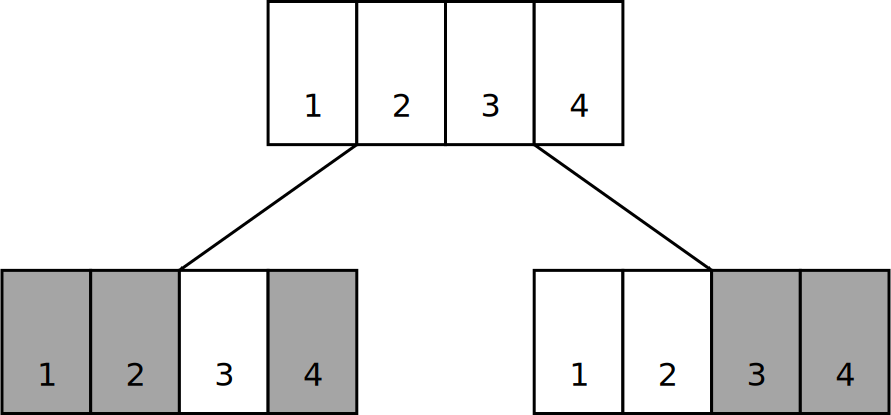
\includegraphics[width=0.5\linewidth]{images/cover_choice.pdf}
    \caption{When boards 1 to 4 are all uncovered, and a 7 is rolled, there are two possible valid coverings - covering boards 1, 2 and 4 (on the left), and covering boards 3 and 4 (on the right).}
    \label{cs1:cover_choice}
\end{figure}

Intuitively, this suggests that lower numbered boards are more valuable later in the game, since they increase the set of possible die rolls that a player can roll without ending the game. From this intuition, we develop two potential strategies for playing Shut the Box. The \emph{high-board strategy} is the strategy where the player always elects to cover the highest number board at each stage, while the \emph{low-board strategy} is the converse, where the player always elects to cover the lowest numbered boards at each stage.

When evaluating the effectiveness of these strategies, model checking is a suitable strategy. Since these strategies are deterministic, we may define DTMCs that model Shut the Box under these strategies, define the score of the game as a reward structure, and evaluate the expected score when the game terminates. However, we are also interested in the \emph{optimal} strategy - that is, the strategy which maximises the expected score of Shut the Box. Trying to enumerate and consider every possible strategy would be challenging, both conceptually and computationally. Instead, we consider the case where \emph{no} strategy is defined - in other words, an entirely nondeterministic strategy - and derive an optimal strategy from here. In order to achieve this, we consider a generalisation of a DTMC which supports nondeterminism.

\section{Background}
\label{cs1:stb_background}

We start by introducing Markov decision processes (MDPs) as described in \cite{forejt_automated_2011}, which are generalisations of DTMCs allowing for actions to be taken at each state, each leading to different probabilistic transitions between states. We then consider adversaries - resolutions of nondeterministic choice in MDPs - and briefly discuss how optimal adversaries are computed.

\subsection{Markov decision processes}
\label{cs1:mdps}
First, we define an MDP as a modification of a DTMC.

\begin{definition}
\label{cs1:def_mdps}

A Markov decision process (MDP) is a tuple $(S, \bar{s}, \mathbf{Steps}, L)$, where $S$, $\bar{s}$ and $L$ have the same meanings as in Definition \ref{back:dtmc}. $\mathbf{Steps} : S \rightarrow 2^{Act \times Dist(S)}$ is the new transition probability function, where states are mapped to a set of pairs of actions and discrete probability distributions, where $Act$ represents the set of actions the player can take.

\end{definition}

For example, in a game of Shut the Box, $Act$ is the set of possible subsets of boards that the player can cover (such as the action of covering boards 3 and 5 simultaneously). Hence, $\mathbf{Steps}$ maps each state, including the current die value and the current set of uncovered boards, to the set of all possible covering arrangements along with the associated state transition.

Note here that, in general, a state may be associated to more than one action-distribution pair. Indeed, this is where nondeterminism is introduced into the MDP. In order to resolve this nondeterminism, we introduce the concept of adversaries.

\begin{definition}
\label{cs1:adversaries}

Given a \emph{finite} path $\omega = s_0 \rightarrow s_1 \rightarrow \dots \rightarrow s_n$, an adversary is a function $\sigma$ which maps each finite path to an action-distribution pair, more specifically an element of $\mathbf{Steps(s_n)}$.

\end{definition}

A key remark on this definition is that adversaries make decisions depending on the entire execution history up to and including the state $s_n$, not just the state $s_n$ itself. However, we primarily consider \emph{memoryless adversaries}, where the adversary always picks the same choice in a given state. In particular, this adversary can be viewed as a map from states to action-distribution pairs, as opposed to a map from finite paths to action-distribution pairs. Throughout the remainder of the dissertation, we only consider memoryless adversaries unless stated otherwise.

When an MDP is considered under an adversary, nondeterministic choice is resolved, and a DTMC is obtained. Hence, under a specific adversary, we can apply the model checking techniques introduced in Section \ref{back:prob_mod_check} to evaluate properties of an MDP.

Note that adversaries are often referred to using other names, depending on context, such as schedulers or policies. Throughout this dissertation, by convention we refer to adversaries when discussing the concept over general MDPs, and refer to strategies in the context of a particular game (analogous to a human developing a strategy while playing a game).

We defer discussion on how adversaries are generated until Section \ref{cs1:adversary_gen}. For now, we discuss how optimal values of probabilistic reachability properties are computed, then modify this process in order to provide an adversary which obtains this optimal value.

\subsection{Probabilistic reachability in MDPs}
\label{cs1:prob_reach_mdps}

In a similar manner to Section \ref{back:check-reach}, given an atomic proposition $a$, we define $T$ to be the set of states in some MDP $\mathcal{M}$ where $a$ holds.

Since MDPs allow for nondeterminism, we must consider a minimum and maximum probability of reaching $T$, over all possible resolutions of nondeterminism. More precisely, for some atomic proposition $a$, we denote these probabilities as $\mathbf{P}_{min}=? [\mathbf{F} \; a]$ and $\mathbf{P}_{max}=? [\mathbf{F} \; a]$ respectively. In order to calculate these probabilities, we introduce a method known as \emph{value iteration}. This method computes a sequence $(x^n_s)_{n \in \mathbb{N}}$, denoting the probability of reaching $T$ from a given state $s$ within $n$ steps. This sequence then converges to an optimal value, yielding a reasonable approximation of the optimal value for large enough $n$.

First, we perform precomputation of several sets of states, very similarly to precomputation of $S^{yes}$ and $S^{no}$ in Definition \ref{back:S_yes}, where the minimum or maximum reachability probabilities are either 0 or 1. The details of these constructions are omitted and described further in Section 4.1 of \cite{forejt_automated_2011}. More formally, these precomputed sets are defined as follows:

\begin{definition}
\label{cs1:yes_no}

For a given MDP $\mathcal{M}$, with state space $S$ and atomic proposition $a$:

\begin{itemize}
    \item $S^{yes}_{min}$ is the set of states where $a$ eventually holds with probability 1, regardless of any nondeterministic choice.
    \item $S^{no}_{min}$ is the state of states where $a$ never holds in any subsequent reachable state, for some resolution of nondeterminism.
    \item $S^{yes}_{max}$ is the set of states where $a$ eventually holds with probability 1, for some resolution of nondeterminism.
    \item $S^{no}_{max}$ is the state of states where $a$ never holds in any subsequent reachable state, regardless of any nondeterministic choice.
\end{itemize}
\end{definition}

For convenience, we also introduce alternative notation for describing the probability of a transition under a given action.

\begin{definition}
\label{cs1:alt_trans_fn}

For an MDP $\mathcal{M}$, where $s$ and $s'$ are states in $mathcal{M}$, $a$ is an action, and $Steps$ is the transition probability function, denote $\delta (s, a)(s')$ as the probability of transitioning from $s$ to $s'$ under action $a$.
\end{definition}

We are now ready to define value iteration for calculating the minimum reachability probability for a set of target states $T$, via defining each element in the sequence $(x^n_s)_{n \in \mathbb{N}}$.

\begin{definition}
\label{cs1:value_iteration}

Given an MDP $\mathcal{M}$, with precomputed sets of states as described in Definition \ref{cs1:yes_no}, we have that:

\begin{equation*}
x^n_s = \begin{cases}
        1 & s \in S^{yes}_{min} \\
        0 & s \in S^{no}_{min} \\
        0 & s \notin (S^{yes}_{min} \cup S^{no}_{min}) \; \text{and} \; n=0 \\
        min_{a \in Act} \sum_{s' \in S}\delta(s,a)(s') \cdot x^{n-1}_{s'} & \text{otherwise} \\
    \end{cases}
\end{equation*}

This sequence may be modified to calculate the maximum reachability property via replacing "min" with "max".
\end{definition}

Using this method,

\subsection{Adversary generation}
\label{cs1:adversary_gen}

When generating adversaries for optimal values of a particular property, we utilise slightly different methods for computing maximum and minimum values. In both cases, since we consider memoryless adversaries, we can generate adversaries by mapping each state to a particular action.

\section{Analysis (3 pages)}

Collect some data, show the results.

\hrule

\Blindtext

\Blindtext

\Blindtext

\section{Evaluation(2 pages)}

The key section - use the results from model checking to answer questions about the game (for instance, to examine the difficulty and/or complexity of a game).

\hrule

\Blindtext

\Blindtext